\documentclass[fleqn,12pt]{article}

\usepackage[utf8]{inputenc}
\usepackage[T1]{fontenc}
\usepackage{mathtools} %loads amsmath
\usepackage{amsthm}
\usepackage{amsfonts}
\usepackage{amsmath}
\usepackage{amssymb}
\usepackage{graphicx}
\usepackage{tikz}
\usetikzlibrary{arrows,automata,positioning}
\usepackage{arydshln}
\usepackage{stmaryrd}
\usepackage{pdflscape}
\usepackage{rotating}
\usepackage[margin=2cm]{geometry}
\usepackage[font=small,labelfont=bf,tableposition=top]{caption}

\tikzset{initial text={}}

\usepackage{fancyhdr}
\setlength{\headheight}{26pt}
\pagestyle{fancy}
\lhead{Static Program Analysis WS 2016/17 -- Series 07 \\ \small{Igor Dudschenko (296764), Oliver Westphal (358321)}}
\rhead{}

\newcommand\dbrackets[1]{\llbracket #1 \rrbracket}

\setlength{\parindent}{0cm}
\newcommand\note[1]{\textcolor{red}{#1}}

\begin{document}
\section*{Exercise 1}
\subsection*{a)}
Given:
$$\text{Galois Connections: } (L_1, \alpha_1, \gamma_1, M_1) \text{ and } (L_2, \alpha_2, \gamma_2, M_2)$$
$$(L_1, \alpha_2 \circ \alpha_1, \gamma_1 \circ \gamma_2,  M_2) \text{ is a Galois connection if } M_1 = L_2$$

To show:

$$\forall l_1 \in L_1: l_1 \sqsubseteq_{L_1} \gamma_1(\gamma_2(\alpha_2(\alpha_1(l_1)))) \text{ and:}$$
$$\forall m_2 \in M_2: \alpha_2(\alpha_1(\gamma_1(\gamma_2(m_2))))  \sqsubseteq_{M_2} m_2 \text{, for: } L_2 = M_1$$

Proof:
Since we know that $(L_1, \alpha_1, \gamma_1, M_1)$ and $(L_2, \alpha_2, \gamma_2, M_2), 
(L_1, \alpha_2 \circ \alpha_1, \gamma_1 \circ \gamma_2,  M_2)$ are Galois connections, we also know that $(L_1, \sqsubseteq_{L_1})$, $(L_2, \sqsubseteq_{L_2})$, $(M_1, \sqsubseteq_{M_1})$ and $(M_2, \sqsubseteq_{M_2})$ are complete Lattices, the following has to hold:

$$\alpha_1:L_1 \rightarrow M_1 \text{ and } \alpha_1:L_1 \rightarrow L_2$$
$$\gamma_2:M_2 \rightarrow L_2 \text{ and } \gamma_2:M_2 \rightarrow M_1$$
$$\alpha_2:L_2 \rightarrow M_2 \text{ and } \alpha_2:M_1 \rightarrow M_2$$
$$\gamma_1:M_1 \rightarrow L_1 \text{ and } \gamma_1:L_2 \rightarrow L_1$$
And:
$$\forall l_1 \in L_1:l_1\sqsubseteq_{L_1} \gamma_1(\alpha_2(l_1)) \sqsubseteq_{L_1} \gamma_1(\gamma_2(\alpha_2(l_1))) \sqsubseteq_{L_1} \gamma_1(\gamma_2(\alpha_2(\alpha_1(l_1))))$$
$$\forall m_2 \in M_2:\alpha_2(\gamma_2(m_2))\sqsubseteq_{M_2} \alpha_2(\gamma_1(\gamma_2(m_2)))\sqsubseteq_{M_2} \sqsubseteq_{M_2} \alpha_2(\alpha_1((\gamma_1(m_2))))\sqsubseteq_{M_2} m_2$$

\subsection*{b)}

$\alpha$:
$$\forall l \in L,\forall m \in M: \alpha_1(l) \sqsubseteq_{L} m$$
$$\forall l \in L,\forall m \in M: \alpha_2(l) \sqsubseteq_{L} m$$
$$\Rightarrow \forall l \in L,\forall m \in M: \alpha(l) \sqsubseteq_{L} m$$

$\gamma$:

$$\forall m \in M: \gamma_1(m_1) \sqsubseteq_L \gamma(m) \text{ and: } \gamma_2(m_2) \sqsubseteq_L \gamma(m)$$

\section*{Exercise 2}
\subsection*{a)}

Proof by Contradiction:\\
Assume that there exists a $l \in 2^{\mathbb{Z}}$, such that $\forall m \in M:\alpha(\gamma(m)) \sqsupset_M m$.\\
Than $\gamma(m) \sqsubseteq \mathbb{Z}$, then $l$ can only exist if $l=\gamma(m)$ and $\alpha(l)\ni {-2,-1,0,1,2}$, since $\mathbb{N}_{even} \cup \mathbb{N}_{odd} \cup -\mathbb{N}_{odd} \cup -\mathbb{N}_{even} \cup {0}=\mathbb{Z}$. And therefore there does not exist a $l \in 2^{\mathbb{Z}}$, such that $\forall m \in M:\alpha(\gamma(m)) \sqsupset_M m$

$$\Rightarrow \forall l \in L: l \sqsubseteq_{L} \gamma(\alpha(l))$$

Assume that there exists a $m \in 2^{-2,-1,0,1,2}$, such that $\forall l \in L:l \sqsupset_L \gamma(\alpha(l))$.\\
Than $\alpha(l) \sqsubseteq {-2,-1,0,1,2}$, then $m$ can only exist if $m=\alpha(l)$ and $\gamma(m)\sqsupset \bigcup_{p \in P}\{p \cdot n | n \in \mathbb{Z}_{>0}\}$, since $p \in \mathbb{Z} \text{ and } n \in \mathbb{Z}_{>0} \Rightarrow \bigcup_{p \in P}\{p \cdot n | n \in \mathbb{Z}_{>0}\} \sqsubseteq \mathbb{Z}$. And therefore there does not exist a $m \in 2^{-2,-1,0,1,2}$, such that $\forall l \in L:l \sqsupset_L \gamma(\alpha(l))$

$$\Rightarrow \forall l \in L:l \sqsubseteq_L \gamma(\alpha(l))$$
\subsection*{b)}

$(2^{\Sigma^{*}},\alpha,\gamma,2^{Q})$ is not a Galois connection. Example:
$$\mathcal{U},Q={q_3,q_4},L_b=\{(a+b+c)^* \cdot (ab+ba)\}:$$

\begin{tikzpicture}[shorten >=1pt,node distance=2cm,on grid,auto] 
   \node[state,initial] (q_0)   {$q_0$}; 
   \node[state] (q_1) [above right=of q_0] {$q_1$}; 
   \node[state] (q_2) [below right=of q_0] {$q_2$}; 
   \node[state,accepting] (q_3) [right=of q_1] {$q_3$}; 
   \node[state,accepting] (q_4) [right=of q_2] {$q_4$}; 
    \path[->] 
    (q_0) edge  [bend left = 45] node {a} (q_1)
          	edge  node {b} (q_2)
	edge [loop below] node {c} ()
    (q_1) edge  node  {b} (q_3)
          	edge [loop above] node {a} ()
	edge  node {c} (q_0)
    (q_2) edge  node {a} (q_4) 
          	edge [loop below] node {b} ()
	edge [bend left = 15] node  {c} (q_0)
    (q_3) edge [bend right = 15]node {a} (q_4) 
          	edge  node {b} (q_2)
	edge [bend left = 15] node  {c} (q_0)
    (q_4) edge[bend right = 30] node {b} (q_3) 
          	edge  node {a} (q_1)
	edge [bend right = 15] node  {c} (q_0);
\end{tikzpicture}
Than we use the following: $\alpha(L_b)={q1}$, for $w=ab$ and now $\gamma(\alpha(L_b)) = \{(a+b+c)^* \cdot {ab}\} \sqsubseteq \{(a+b+c)^* \cdot {ab+ba}\}$, which shows that this can not be a Galois connection. 
\subsection*{c)}

\subsection*{d)}

\subsection*{e)}

\end{document}
